% Sample Graph Visualization
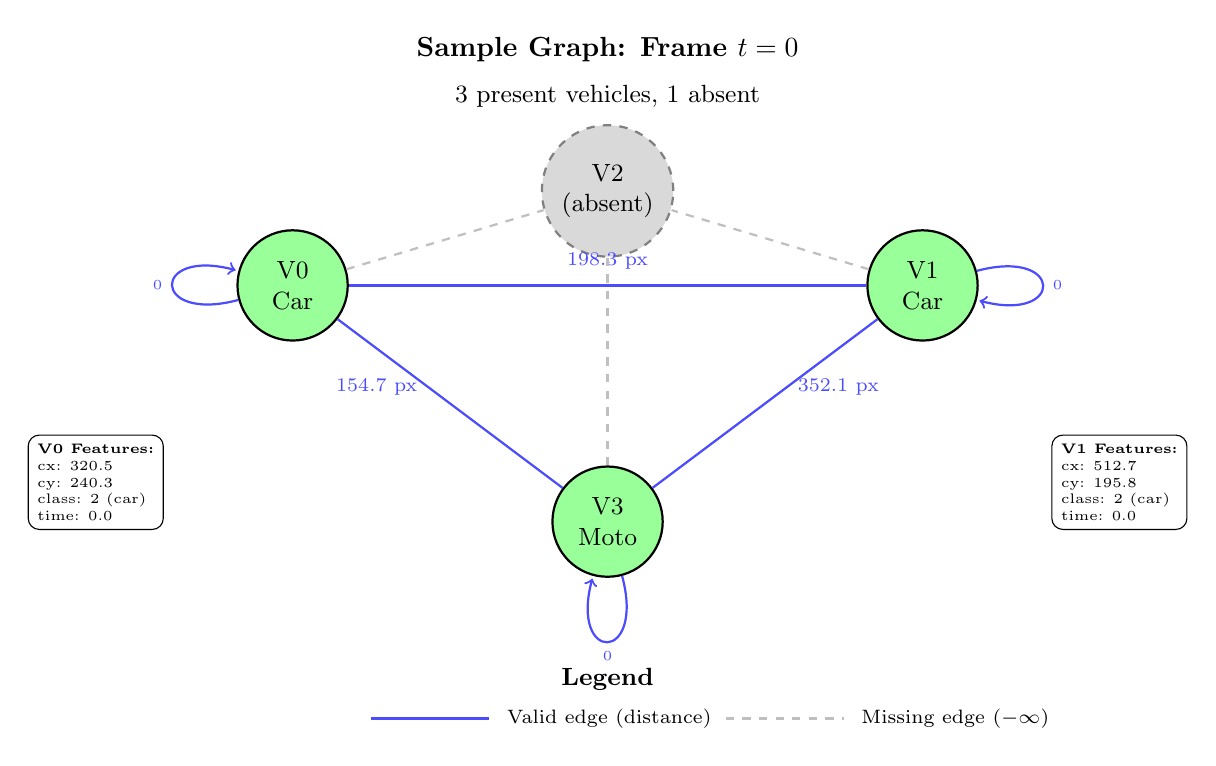
\begin{tikzpicture}[
    vertex/.style={
        circle,
        draw=black,
        thick,
        minimum size=1.4cm,
        font=\small,
        align=center
    },
    present/.style={vertex, fill=green!40},
    absent/.style={vertex, fill=gray!30, dashed, draw=gray},
    edge/.style={thick, blue!70},
    missing/.style={thick, dashed, gray!50}
]

% Title
\node[font=\bfseries] at (5, 6) {Sample Graph: Frame $t=0$};
\node[font=\small] at (5, 5.4) {3 present vehicles, 1 absent};

% Present nodes - wider spacing to avoid overlaps
\node[present] (v0) at (1, 3) {V0\\Car};
\node[present] (v1) at (9, 3) {V1\\Car};
\node[present] (v3) at (5, 0) {V3\\Moto};

% Absent node - moved up to avoid edge label overlap
\node[absent] (v2) at (5, 4.2) {V2\\(absent)};

% Edges between present nodes with adjusted label positions
\draw[edge] (v0) -- node[above, font=\scriptsize, pos=0.5, yshift=2pt] {198.3 px} (v1);
\draw[edge] (v0) -- node[left, font=\scriptsize, pos=0.4] {154.7 px} (v3);
\draw[edge] (v1) -- node[right, font=\scriptsize, pos=0.4] {352.1 px} (v3);

% Missing edges to absent node
\draw[missing] (v0) -- (v2);
\draw[missing] (v1) -- (v2);
\draw[missing] (v3) -- (v2);

% Self-loops (indicated)
\draw[edge, ->] (v0) edge[loop left] node[font=\tiny] {0} (v0);
\draw[edge, ->] (v1) edge[loop right] node[font=\tiny] {0} (v1);
\draw[edge, ->] (v3) edge[loop below] node[font=\tiny] {0} (v3);

% Node info boxes - positioned outside the graph
\node[font=\tiny, align=left, fill=white, draw, rounded corners] at (-1.5, 0.5) {
    \textbf{V0 Features:}\\
    cx: 320.5\\
    cy: 240.3\\
    class: 2 (car)\\
    time: 0.0
};

\node[font=\tiny, align=left, fill=white, draw, rounded corners] at (11.5, 0.5) {
    \textbf{V1 Features:}\\
    cx: 512.7\\
    cy: 195.8\\
    class: 2 (car)\\
    time: 0.0
};

% Legend
\node[font=\small\bfseries] at (5, -2) {Legend};
\draw[edge] (2, -2.5) -- (3.5, -2.5);
\node[font=\scriptsize, right] at (3.6, -2.5) {Valid edge (distance)};

\draw[missing] (6.5, -2.5) -- (8, -2.5);
\node[font=\scriptsize, right] at (8.1, -2.5) {Missing edge ($-\infty$)};

\end{tikzpicture}
